\section{Projet Gestion des Recours}
\subsection{Introduction}
\subsubsection{Contexte et présentation}
Dans le processus de passation ou d'exécution des marchés publics au Togo, des différends peuvent surgir en raison de violations des textes ou des clauses contractuelles. Après un premier recours auprès de l'autorité contractante concernée, les requérants peuvent saisir l'ARCOP pour un examen approfondi.

\subsubsection{Objectifs}
Le projet vise à optimiser le suivi et le traitement interne des recours déposés auprès de l'ARCOP, en facilitant leur gestion par les différents acteurs impliqués.

\subsection{Spécifications fonctionnelles}
\subsubsection{Filtrage des recours}
\begin{itemize}
    \item \textbf{Entre deux dates} : Filtrage par période de dépôt
    \item \textbf{Par décision} : Filtrage selon les décisions rendues
    \item \textbf{Autres critères} : Filtrage par requérant, autorité contractante, etc.
\end{itemize}

\subsubsection{Enregistrement et mise à jour}
Ajout et modification des informations relatives aux recours

\subsubsection{Envoi des mails}
Notifications automatiques pour les recours dont le traitement est en retard

\subsubsection{Vue globale des recours}
\begin{itemize}
    \item Visualisation graphique des recours par type de décision
    \item Filtrage temporel des graphiques
    \item Affichage des recours en cours avec durée écoulée depuis le dépôt
\end{itemize}

\subsection{Cas d'utilisation principaux}
\subsubsection{Description des cas d'utilisation}
\begin{itemize}
    \item \textbf{Enregistrer un recours} : Saisie des informations (requérant, autorité contractante, date de dépôt, objet)
    \item \textbf{Traiter un recours} : Étude (acceptation/rejet) et décision de fond
    \item \textbf{Supprimer un recours} : Possible tant que le recours n'est pas pris en charge
    \item \textbf{Visualiser les recours} : Vue d'ensemble ou détaillée avec filtres
\end{itemize}

\subsubsection{Diagramme de cas d'utilisation}
\begin{figure}[H]
    \centering
    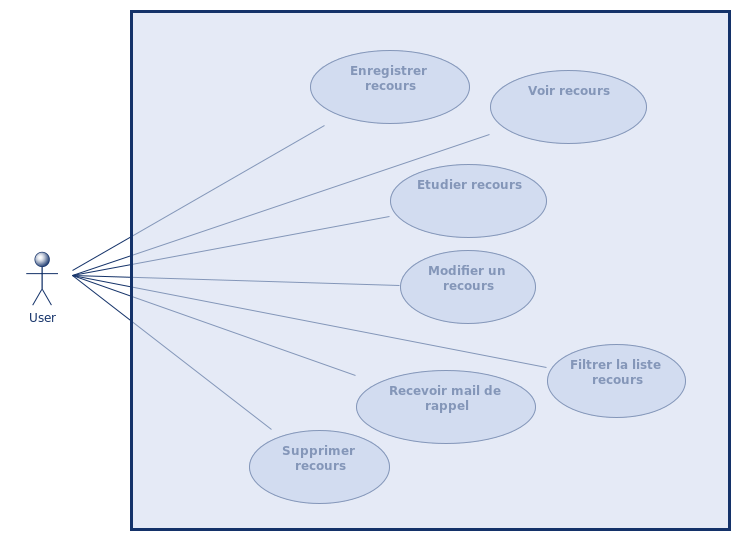
\includegraphics[width=0.8\textwidth]{images/diagrammes/use-cases/Diagramme de cas d'utilisation recours.png}
    \caption{Diagramme de cas d'utilisation Gestion des Recours}
    \label{fig:use_case_gestion_recours}
\end{figure}
